\documentclass[11pt]{article}
\usepackage[margin=1in]{geometry}
\usepackage{amsmath,amssymb}
\usepackage{graphicx}
\usepackage{booktabs}
\usepackage{xcolor}
\usepackage[colorlinks=true,linkcolor=blue,citecolor=blue,urlcolor=blue]{hyperref}
\usepackage{caption}
\captionsetup{font=small,labelfont=bf}
\graphicspath{{figures/}{analysis/}}

\title{\bfseries Certified Penetration-Safety Envelopes for\\
Directed-Energy Area Defense against Adversarial Drone Swarms}
\author{overthelex\\ \small\texttt{github.com/overthelex/hpm-saturation-analysis}}
\date{Working draft --- \today}

\begin{document}
\maketitle

\begin{abstract}
High-power-microwave (HPM) weapons are being fielded as the primary counter to drone swarms,
on the premise that one ``one-to-many'' pulse defeats many targets at once. Whether a given
emplacement actually \emph{holds} against an adversarial swarm---and against which swarm
configurations it fails---is today decided by ad-hoc live-fire demonstrations, not by any
principled guarantee. We import and extend the machinery of \emph{certified robustness} from
machine learning to physical area defense. Given a defense configuration~$d$, we compute a
\emph{certified penetration-safety envelope} $\hat{A}$: a region of attacker configurations
for which the defense provably holds (penetration below a threshold) at a stated statistical
confidence, together with the worst-case adversarial swarm that maximizes penetration. The
obstacle is that the ``input'' is a structured, physically-constrained attack configuration
and the objective is a stochastic, expensive, black-box simulation with a rare-event tail
near the safe region. We combine (i)~level-set active learning of the failure boundary,
(ii)~physics-structured black-box adversarial search, and (iii)~conformal certification with a
rare-event tail estimate. On a calibrated directed-energy counter-swarm simulator we show that
a Gaussian-process surrogate under level-set active learning recovers the failure boundary
using $14\%$ of a dense-grid budget and $79\%$ more accurately than random sampling (E1); that
black-box adversarial search \emph{autonomously rediscovers} two independently-derived
vulnerability modes---a zenith ballistic drop and a target-hardening range collapse---from a
bare ``maximize penetration'' objective (E2); that a distribution-free conformal certificate
yields a certified-safe envelope with valid coverage, zero false-safe region, $93\%$
tightness, and which survives an active adversarial search (E3); and that subset simulation
certifies a small penetration probability $\Pr[\text{leak}\ge\tau]\approx10^{-3}$ that naive
Monte-Carlo cannot resolve (E4); and that Sobol sensitivity attribution identifies the
one-to-many capacity and effective range as the co-dominant design levers (E5). A
quality-diversity joint search finds no cheap third full mode beyond the two hand-derived ones
(E6), while a dedicated sweep shows drone \emph{speed} (up to 600\,km/h) is a genuine partial
third breakthrough axis, scaling the saturation ratio linearly (E7).
\end{abstract}

\section{Introduction}
Cheap drone swarms have shifted the economics of air defense: a \$10k airframe cannot be met
by a \$1M interceptor at scale. High-power-microwave (HPM) directed-energy weapons answer this
with a soft-kill ``one-to-many'' pulse that disables the electronics of every drone in a beam
volume at negligible cost per shot. But directed energy has structural blind spots---a beam
can only point one way at a time (angular saturation), a ring of emitters cannot fire inward
without fratricide, and a soft-kill weapon cannot stop an inert falling mass. Whether a fielded
configuration is \emph{safe} against a determined swarm is currently answered by live-fire
demonstrations that sample a handful of scenarios.

We ask instead for a \emph{guarantee}: a certified region of attacker configurations for which
a given defense provably holds, and the worst-case attack that breaks it. This is precisely the
question \emph{certified robustness} answers for machine-learning classifiers, and
\emph{falsification} answers (partially) for cyber-physical systems. We transfer and adapt that
machinery to physical area defense. Our contributions are: (1)~a formal framework---the
certified penetration-safety envelope and the adversarial-swarm objective for area defense
(\S\ref{sec:formulation}); (2)~a method combining level-set active learning, physics-structured
black-box adversarial search, and conformal certification, for a black-box stochastic defense
simulator (\S\ref{sec:method}); and (3)~empirical validation on a calibrated directed-energy
counter-swarm simulator, including automatic rediscovery of independently-derived adversarial
modes (\S\ref{sec:experiments}).

\section{Related work}
\emph{Certified robustness in ML} (randomized smoothing~\cite{cohen2019}; convex/IBP
certificates~\cite{wong2018}) certifies a classifier over an $L_p$ ball of a fixed input. Our
``input'' is a structured physical attack, the model is a black-box stochastic simulator, and
the perturbation set is a physics-constrained budget. \emph{Falsification of cyber-physical
systems}~\cite{fainekos2009,donze2010} finds \emph{one} counterexample; we compute the
\emph{certified safe set} and verify it. \emph{Stackelberg security games}~\cite{tambe2011}
solve allocation equilibria on discrete structures, not a continuous physics-constrained
penetration boundary. \emph{Counter-UAS / DEW operations research} (salvo models~\cite{hughes1995};
probability of raid annihilation) gives aggregate exchange metrics, not per-configuration
certificates. \emph{Level-set estimation}~\cite{gotovos2013} and \emph{rare-event simulation}
(subset simulation~\cite{aubeck2001}) are our tools; we combine them into a certificate for
adversarial physical defense---the gap we fill.

\section{Problem formulation}\label{sec:formulation}
A defense configuration $d\in\mathcal{D}$ (emitter count, positions, beam half-angle $\theta$,
effective range $R_{\text{eff}}$, engagement cycle $t_c$, one-to-many capacity $n_{\text{cone}}$,
elevation limit, mobility, kinetic budget) and an attack configuration $a\in\mathcal{A}$ (swarm
size $N$, approach geometry, altitude, target hardening $E_{\text{kill}}$, timing) map through a
simulator $S$ to a penetration (leak) fraction under randomness $\omega$:
\begin{equation}
\text{leak}=S(d,a;\omega)\in[0,1],\qquad L(d,a)=\mathbb{E}_\omega[S(d,a;\omega)].
\end{equation}
For a leak threshold $\tau$, the \emph{failure boundary} is
$\partial_\tau(d)=\{a:L(d,a)=\tau\}$, separating the safe region
$A_{\text{safe}}(d)=\{a:L(d,a)<\tau\}$ from the penetrated region. A
\emph{certified penetration-safety envelope} is a set $\hat A\subseteq\mathcal A$ and confidence
$1-\alpha$ with
\begin{equation}
\Pr\!\big[\,\forall a\in\hat A:\ L(d,a)<\tau\,\big]\ \ge\ 1-\alpha,
\end{equation}
the outer probability over the estimation procedure. Dually the \emph{adversarial swarm} is
$a^\ast(d)=\arg\max_{a\in A_{\text{budget}}}L(d,a)$; the defense is certified on
$A_{\text{budget}}$ iff $L(d,a^\ast(d))<\tau$. The difficulty is that $L$ is black-box,
non-differentiable, expensive (each evaluation is a Monte-Carlo of a 3-D agent simulation),
stochastic, and \emph{rare-event} near $A_{\text{safe}}$.

\paragraph{Simulator.} We use an open 3-D time-stepped agent model of directed-energy
counter-swarm engagement (angular/temporal saturation, fratricide no-fire regions, elevation
gap, soft-kill physics, optional kinetic layer), calibrated to open-source parameters and
validated against a closed-form saturation threshold. For a single aperture the model gives a
sharp boundary $\Sigma\equiv S(\theta)\,t_c\,v/(R_{\text{eff}}-R_c)=1$ with
$S(\theta)=1/(1-\cos\theta)$; Fig.~\ref{fig:sat} shows the simulated leak against this boundary.

\begin{figure}[t]
\centering
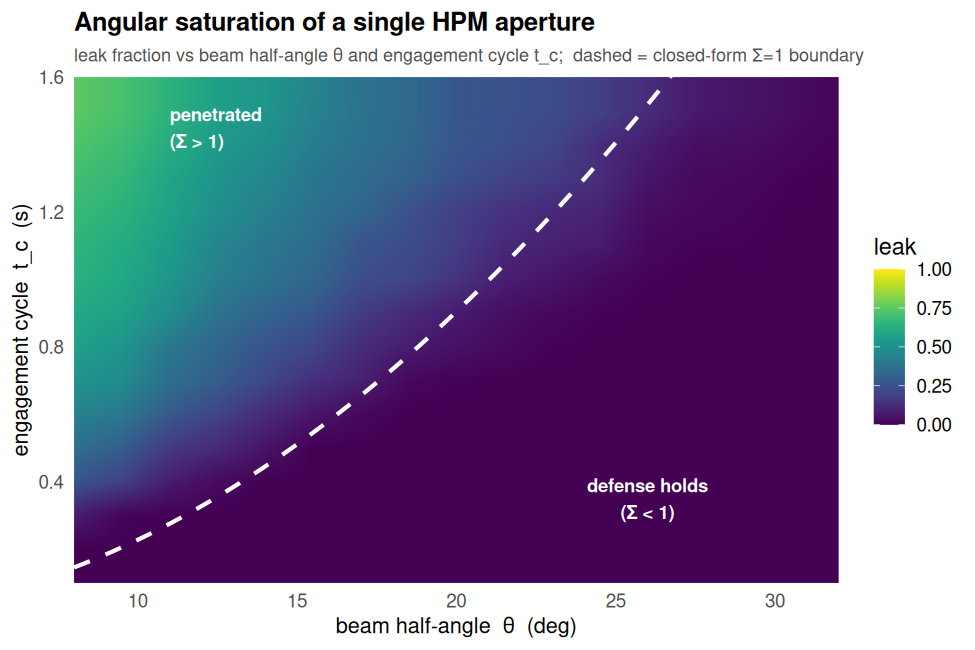
\includegraphics[width=0.72\linewidth]{fig_saturation_phase.png}
\caption{Angular saturation of a single HPM aperture: simulated leak fraction versus beam
half-angle $\theta$ and engagement cycle $t_c$. The dashed curve is the closed-form
$\Sigma=1$ boundary; it coincides with the simulated transition.}
\label{fig:sat}
\end{figure}

\section{Method}\label{sec:method}
\textbf{M1 --- Failure-boundary active learning.} Model $L(d,\cdot)$ with a Gaussian-process
surrogate $\hat G$. Query with a level-set (straddle) acquisition
$1.96\,\sigma(a)-|\mu(a)-\tau|$, concentrating oracle calls on $\partial_\tau$.

\textbf{M2 --- Physics-structured adversarial search.} Find $a^\ast$ by gradient-free
optimization (differential evolution) over $\mathcal A$, respecting physical constraints via
reparameterization---the black-box analogue of a white-box adversarial attack.

\textbf{M3 --- Conformal certification.} From a held-out calibration set, one-sided
split-conformal scores $s_i=y_i-\mu(x_i)$ give a margin $q$ (their
$\lceil(n{+}1)(1-\alpha)\rceil$ order statistic) and a distribution-free upper bound
$U(a)=\mu(a)+q$ with $\Pr[L(a)\le U(a)]\ge1-\alpha$. The certified-safe set is
$\hat A=\{a:U(a)<\tau\}$, verified by an active adversarial search restricted to $\hat A$; a
subset-simulation tail estimate certifies the small penetration probability
$\Pr_\omega[\text{leak}\ge\tau]$.

\section{Experiments}\label{sec:experiments}
We validate on a single-aperture 2-D slice $(\theta,t_c)$ at fixed $R_{\text{eff}}=500$\,m,
$R_c=50$\,m, $v=30$\,m/s, $N=80$, chosen for its closed-form boundary; larger and multi-modal
attack spaces are used in E2.

\subsection{E1 --- surrogate and boundary recovery}
At a tight budget of 24 oracle queries ($14\%$ of a dense $13\times13$ Monte-Carlo grid), the
GP surrogate recovers the failure boundary to $0.038$\,s in $t_c$; level-set active learning is
$79\%$ more accurate on the boundary than same-budget random sampling
(Table~\ref{tab:e1}, Fig.~\ref{fig:e1}).

\begin{table}[h]
\centering
\caption{E1: boundary recovery at 24 queries ($14\%$ of a dense grid).}
\label{tab:e1}
\begin{tabular}{lcc}
\toprule
Metric & Active learning & Random \\
\midrule
Global surrogate RMSE (leak) & 0.027 & 0.037 \\
\textbf{Boundary RMSE} ($t_c$, s) & \textbf{0.038} & \textbf{0.179} \\
\bottomrule
\end{tabular}
\end{table}

\begin{figure}[t]
\centering
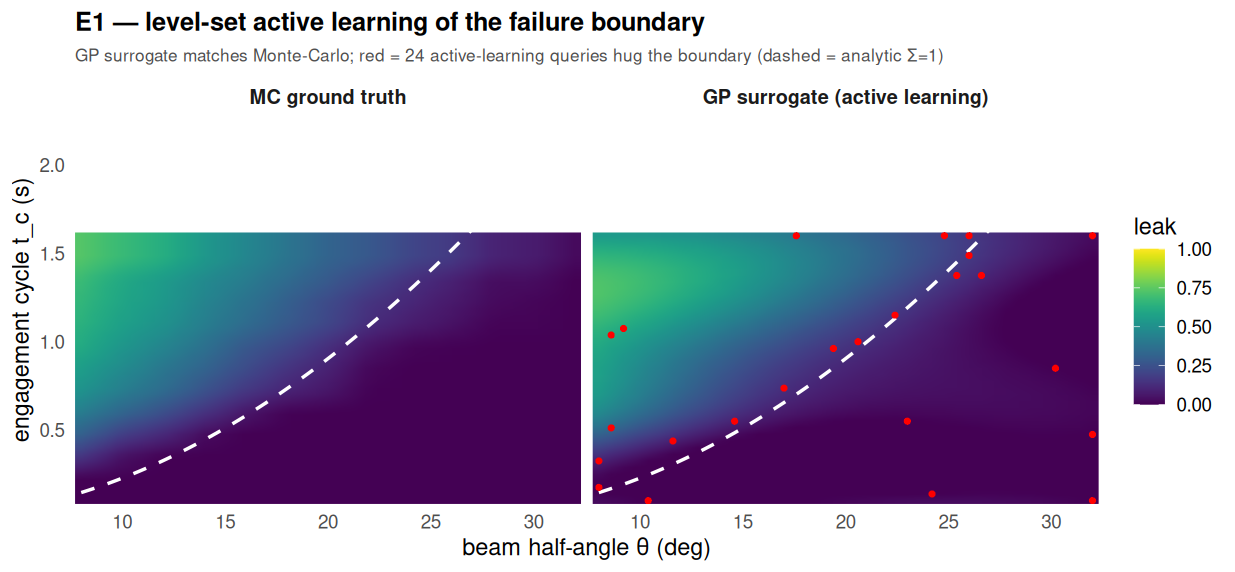
\includegraphics[width=\linewidth]{fig_e1_surrogate.png}
\caption{E1. GP surrogate (right) matches the Monte-Carlo ground truth (left); the 24
active-learning queries (red) cluster along the failure boundary. Dashed: analytic $\Sigma=1$.}
\label{fig:e1}
\end{figure}

\subsection{E2 --- adversarial rediscovery}
Against a calibrated four-emitter defense ($\theta=30^\circ$, $n_{\text{cone}}=49$,
$\text{el}_{\max}=80^\circ$, $R_{\text{eff}}=500$\,m) that holds against a direct attack
(leak $0.000$), black-box search with only a ``maximize penetration'' objective autonomously
rediscovers two independently-derived modes (Fig.~\ref{fig:e2}): (1)~a \emph{zenith ballistic
drop}---climb above the cone-of-silence floor ($869$\,m) and free-fall, immune to soft-kill
(leak~$\to1.000$); (2)~a \emph{hardening/$R_{\text{eff}}$ collapse}---shield the drones
$\sim22$\,dB, collapsing effective range $500\to40$\,m (leak~$\to1.000$). Both were derived
analytically before the search; the optimizer found them with no prior knowledge.

\begin{figure}[t]
\centering
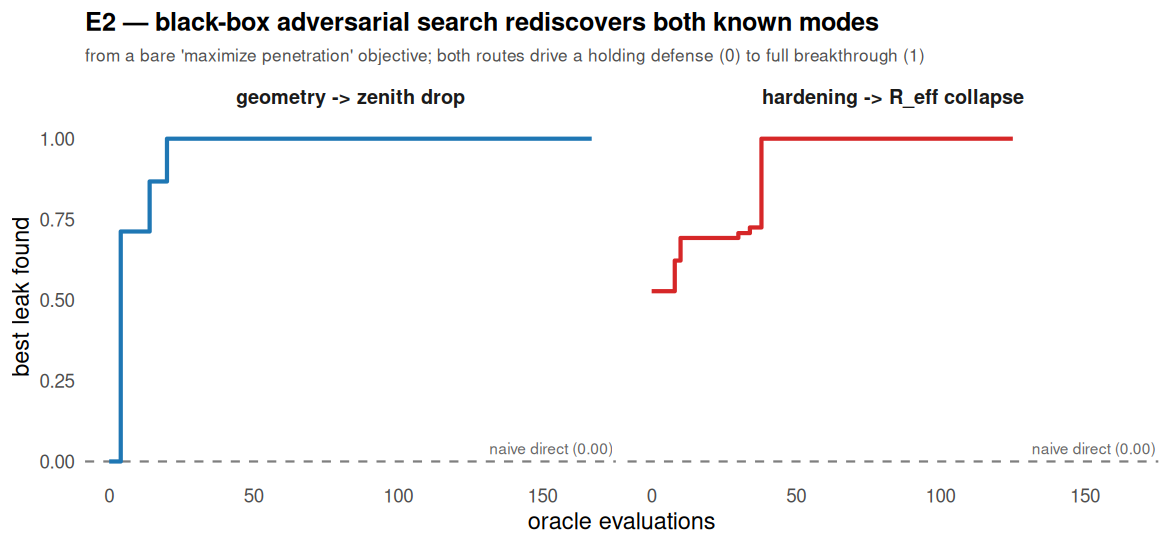
\includegraphics[width=\linewidth]{fig_e2_adversarial.png}
\caption{E2. Best leak found versus oracle evaluations. From a holding defense (dashed, $0$),
each search independently reaches full breakthrough by a distinct route.}
\label{fig:e2}
\end{figure}

\subsection{E3 --- certification}
With $\tau=0.15$ and $1-\alpha=90\%$, the conformal certificate passes all four checks
(Table~\ref{tab:e3}, Fig.~\ref{fig:e3}): valid coverage, no false-safe region, $93\%$
tightness, and an active black-box search restricted to $\hat A$ cannot exceed leak $0.125<\tau$.

\begin{table}[h]
\centering
\caption{E3: conformal certificate ($\tau=0.15$, $90\%$ confidence).}
\label{tab:e3}
\begin{tabular}{lcc}
\toprule
Check & Result & Target \\
\midrule
Coverage (test) & 0.938 & $\ge0.90$ \\
Soundness (false-safe rate) & 0.000 & $\le0.10$ \\
Tightness $|\hat A|/|A_{\text{safe}}|$ & 0.929 & $\to1$ \\
Worst true leak inside $\hat A$ & 0.125 & $<0.15$ \\
\bottomrule
\end{tabular}
\end{table}

\begin{figure}[t]
\centering
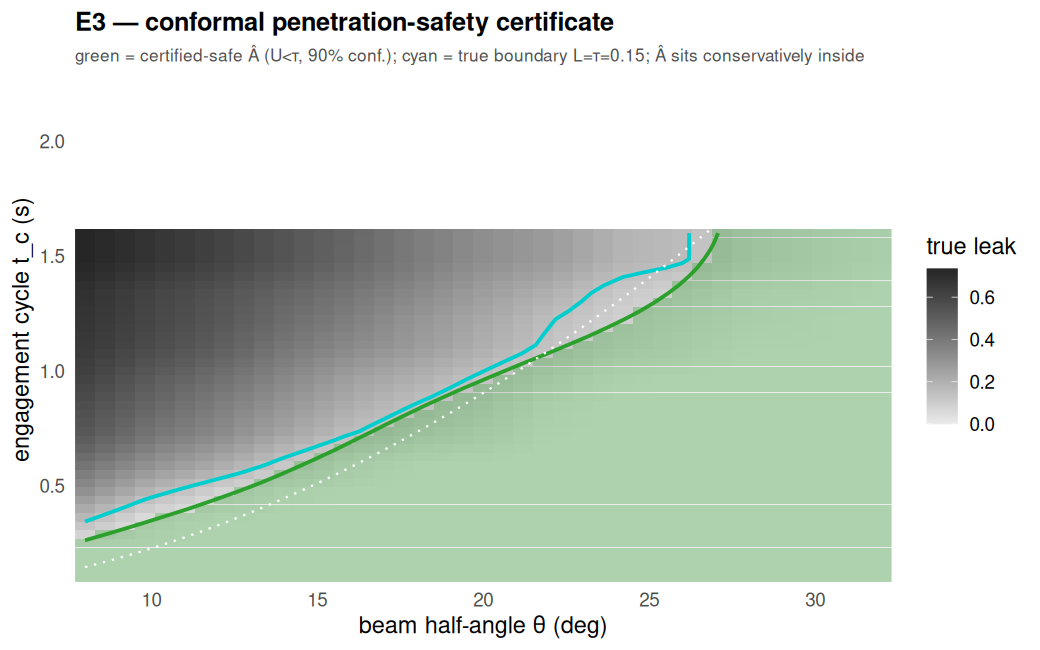
\includegraphics[width=0.72\linewidth]{fig_e3_certificate.png}
\caption{E3. The certified-safe envelope $\hat A$ (green) sits conservatively inside the true
safe region; the conformal boundary $U=\tau$ (green) is a safe margin below the true boundary
$L=\tau$ (cyan), with no false-safe points.}
\label{fig:e3}
\end{figure}

\subsection{E4 --- rare-event tail certification}
Making the randomness explicit ($\omega\in\mathbb{R}^{120}$ perturbing spawn geometry;
hard-step kill so $g(\omega)=\text{leak}(\omega)$ is deterministic), we estimate the tail
$p=\Pr_\omega[\text{leak}\ge\tau]$ by subset simulation (Fig.~\ref{fig:e4}). At a moderate level
where naive Monte-Carlo is reliable, subset simulation agrees within $0.9\times$
($3.0\times10^{-2}$ vs $3.5\times10^{-2}$) using $12\%$ of the budget---validating the
estimator; at a rare level where naive Monte-Carlo sees a single event, subset simulation
resolves $p\approx1.0\times10^{-3}\pm3.7\times10^{-4}$, ${\sim}11\times$ more sample-efficient.

\begin{figure}[t]
\centering
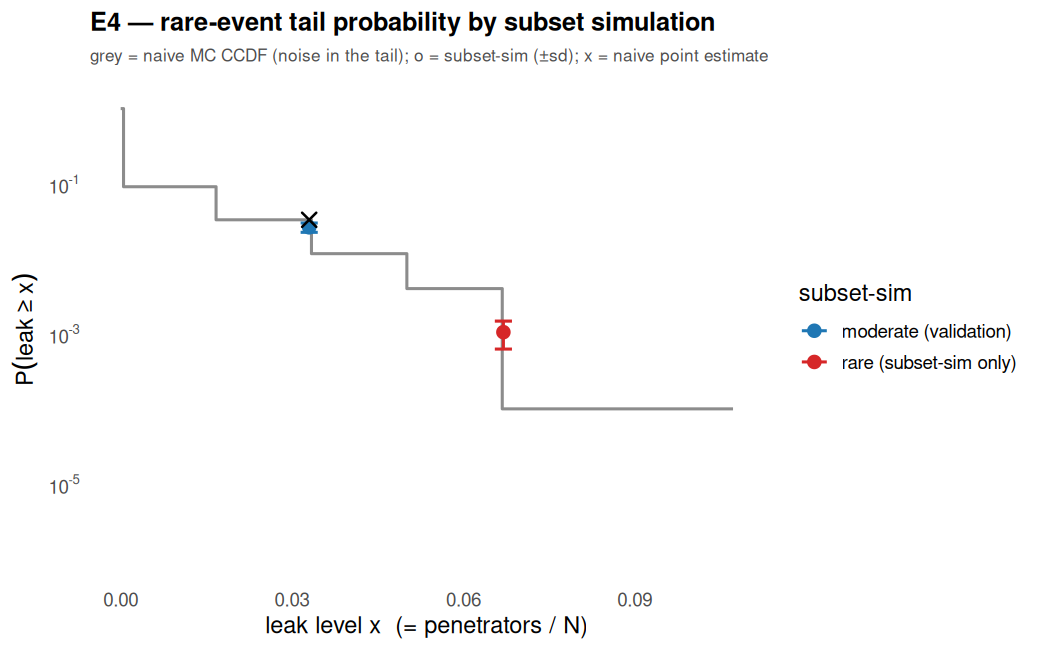
\includegraphics[width=0.68\linewidth]{fig_e4_tail.png}
\caption{E4. Naive Monte-Carlo CCDF (grey) is pure noise in the tail; subset simulation (o,
$\pm$sd) resolves the penetration probability where naive MC has a single sample (\texttt{x}).}
\label{fig:e4}
\end{figure}

\subsection{E5 --- sensitivity attribution and design guidance}
Global (variance-based) Sobol indices identify what governs penetration of the hectare
defense, turning the certificate into design guidance. Over six parameters (Saltelli $N=64$,
$512$ configurations, direct attack), the one-to-many capacity $n_{\text{cone}}$ and the
effective range $R_{\text{eff}}$ are statistically \emph{co-dominant} (overlapping confidence
intervals), followed by the engagement cycle $t_c$; beam half-angle and approach speed are
second-order in this regime (Table~\ref{tab:e5}, Fig.~\ref{fig:e5}). The guidance is to invest
first in $n_{\text{cone}}$ and $R_{\text{eff}}$; the adversary's strongest lever is collapsing
$R_{\text{eff}}$ via drone hardening ($R_{\text{eff}}\propto1/E_{\text{kill}}$), the
quantitative confirmation of the E2 hardening mode.

\begin{table}[h]
\centering
\caption{E5: Sobol indices for hectare-defense penetration (direct attack, $N=64$).}
\label{tab:e5}
\begin{tabular}{lcc}
\toprule
Parameter & $S_1$ & $S_T$ \\
\midrule
$n_{\text{cone}}$ (one-to-many) & 0.273 & \textbf{0.385} \\
$R_{\text{eff}}$ (range / hardening) & 0.332 & \textbf{0.374} \\
$t_c$ (cycle) & 0.178 & 0.306 \\
$N$ (swarm size) & 0.150 & 0.113 \\
$v$ (speed) & $-0.024$ & 0.082 \\
$\theta$ (beam width) & $-0.003$ & 0.041 \\
\bottomrule
\end{tabular}
\end{table}

\begin{figure}[t]
\centering
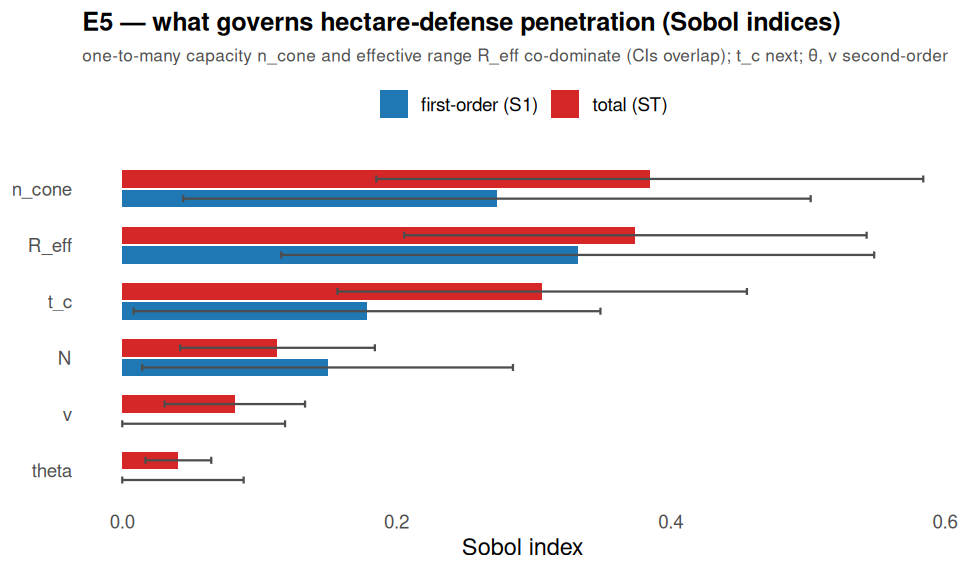
\includegraphics[width=0.72\linewidth]{fig_e5_sensitivity.png}
\caption{E5. Sobol first-order ($S_1$) and total ($S_T$) indices with confidence intervals;
$n_{\text{cone}}$ and $R_{\text{eff}}$ co-dominate the penetration variance.}
\label{fig:e5}
\end{figure}

\subsection{E6/E7 --- joint mode search and the speed axis}
Two further experiments probe for failure modes beyond the two hand-derived ones. \textbf{E6}
runs a quality-diversity (MAP-Elites) \emph{joint} search over a combined attack genome
(altitude, hardening, elevation, speed, azimuth seam-routing), mapping diverse
high-penetration strategies rather than a single optimum (Fig.~\ref{fig:e6}). The map shows
two full-breakthrough ridges---the zenith drop and the hardening collapse---and \emph{no}
cheap third full mode: the direct-and-soft corner holds (leak $\approx0.09$). \textbf{E7}
isolates drone \emph{speed} (up to $167$\,m/s $=600$\,km/h): since
$\Sigma\propto t_c\,v$, fast drones shrink the engagement window, and speed is a genuine but
\emph{partial} third axis---a $600$\,km/h soft, direct swarm erodes a hectare that holds
against $2000$ slow drones, with strength set by the engagement cycle $t_c$
(Fig.~\ref{fig:e7}). Both experiments run the simulator across all CPU cores
(embarrassingly parallel; ${\sim}10\times$ wall-clock, bit-identical results).

\begin{figure}[t]
\centering
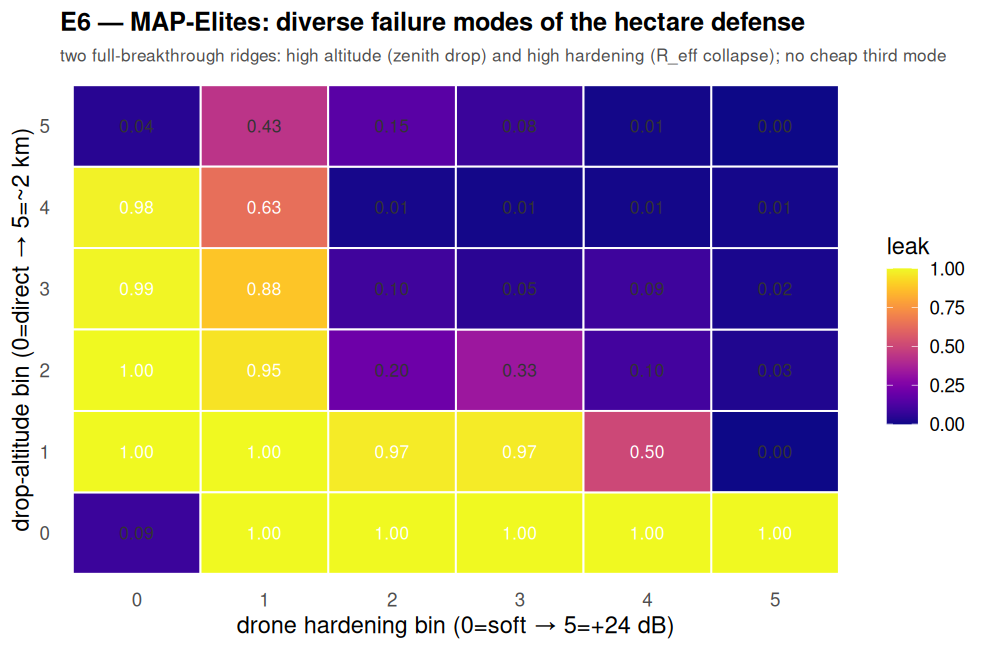
\includegraphics[width=0.66\linewidth]{fig_e6_modes.png}
\caption{E6. MAP-Elites diversity map (drop altitude $\times$ hardening): two full-breakthrough
ridges (zenith drop, hardening collapse) and no cheap third mode.}
\label{fig:e6}
\end{figure}

\begin{figure}[t]
\centering
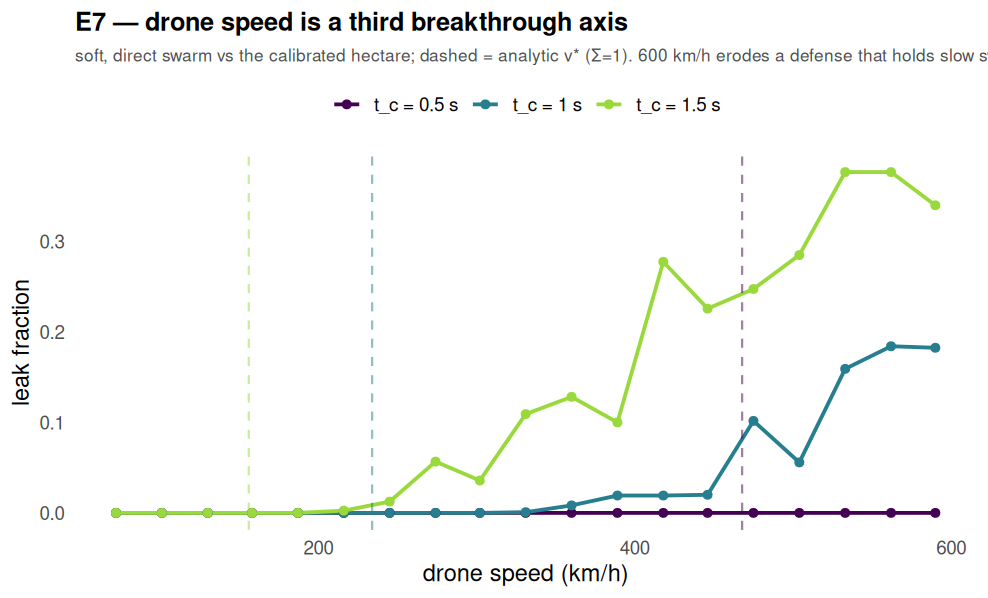
\includegraphics[width=0.66\linewidth]{fig_e7_speed.png}
\caption{E7. Leak vs drone speed for three engagement cycles; a $600$\,km/h swarm penetrates a
defense that holds slow swarms. Dashed: analytic single-aperture $v^\ast$ (a lower bound).}
\label{fig:e7}
\end{figure}

\section{Discussion and limitations}
The certificate is \emph{with respect to the simulator model}; parameters are
order-of-magnitude on open sources, and the method is fidelity-agnostic---it transfers verbatim
to a higher-fidelity simulator. Conformal coverage here is \emph{marginal} (per-point); a
$\forall a\in\hat A$ set-guarantee needs a union/rare-event strengthening, for which E4 is the
ingredient. Validation is on a 2-D slice; scaling certification to high-dimensional attack
spaces (structured decomposition; certify per scenario family) is the main open problem.
Ethically, the work is framed defensively---it certifies that a defense holds or reveals a gap
to close---and abstracts away from any specific fielded weapon.

\section{Conclusion}
We recast ``does this air defense hold?'' as a certification problem and transferred
certified-robustness machinery to physical directed-energy area defense. A GP surrogate under
level-set active learning recovers the failure boundary sample-efficiently; black-box
adversarial search autonomously rediscovers real vulnerability modes; a conformal certificate
yields a verified penetration-safety envelope; subset simulation certifies its rare-event
tail; and Sobol attribution turns it into design guidance. The pieces compose into a pipeline
that turns an engineering simulation into a provable, adversarially-verified statement about a
physical defense.

\begin{thebibliography}{9}
\small
\bibitem{cohen2019} J.~Cohen, E.~Rosenfeld, Z.~Kolter. Certified adversarial robustness via
randomized smoothing. \emph{ICML}, 2019.
\bibitem{wong2018} E.~Wong, Z.~Kolter. Provable defenses via the convex outer adversarial
polytope. \emph{ICML}, 2018.
\bibitem{gotovos2013} A.~Gotovos, N.~Casati, G.~Hitz, A.~Krause. Active learning for level set
estimation. \emph{IJCAI}, 2013.
\bibitem{aubeck2001} S.-K.~Au, J.~Beck. Estimation of small failure probabilities in high
dimensions by subset simulation. \emph{Prob. Eng. Mech.}, 16(4), 2001.
\bibitem{fainekos2009} G.~Fainekos, G.~Pappas. Robustness of temporal logic specifications for
continuous-time signals. \emph{Theor. Comput. Sci.}, 2009.
\bibitem{donze2010} A.~Donz\'e. Breach, a toolbox for verification and parameter synthesis of
hybrid systems. \emph{CAV}, 2010.
\bibitem{tambe2011} M.~Tambe. \emph{Security and Game Theory}. Cambridge Univ. Press, 2011.
\bibitem{hughes1995} W.~Hughes. A salvo model of warships in missile combat. \emph{Naval
Research Logistics}, 42(2), 1995.
\end{thebibliography}

\end{document}
